%!TEX root = ../iotpaper.tex

\subsection{Experimental Platform}
\label{sec:Tooling}

Our experiments focus on multiple mobile devices with 3-axis accelerometers: two iPhone 6, one iPhone 6s, Nexus 5 (Android). For ease of implementation, each device communicates with a laptop running MATLAB, and the laptop takes and compares the accelerometer data from each device. We also compare performance against a classic Pebble smartwatch's accelerometer data. The data flow is shown in \autoref{fig:hardware}.

\begin{figure}[!tb]
\centering
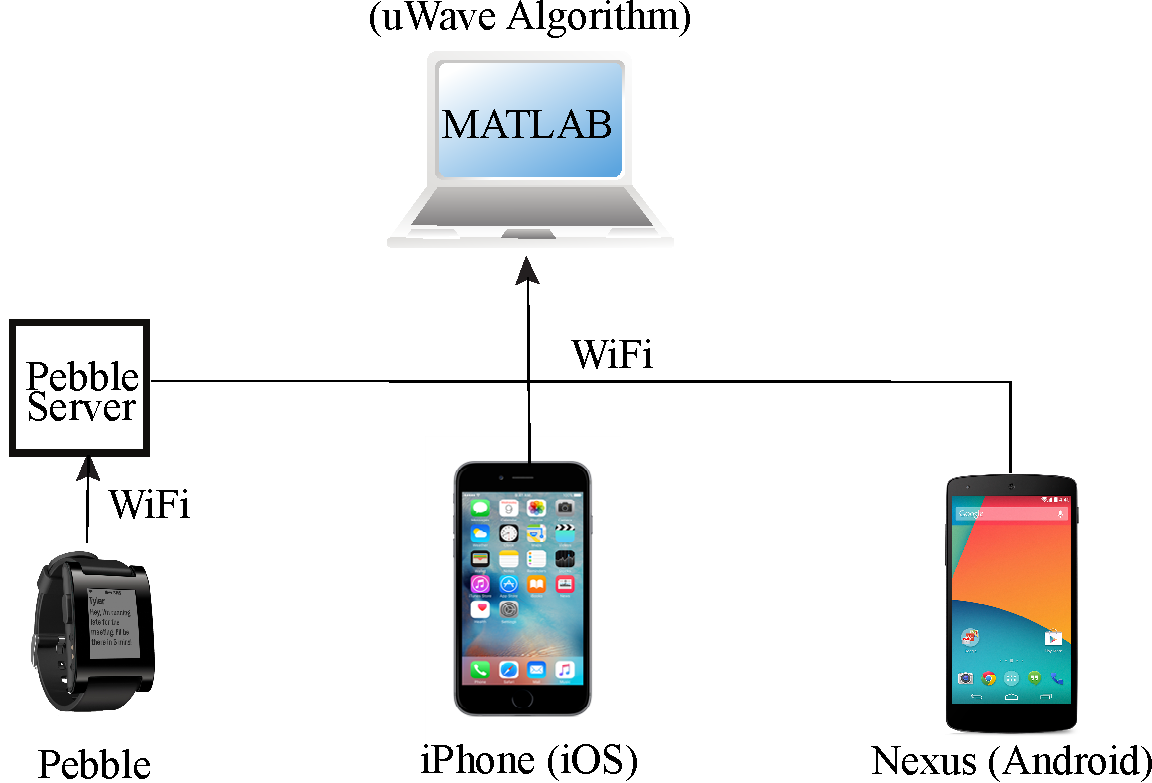
\includegraphics[width=0.9 \linewidth]{./figures/hardware_composition.pdf}
\caption{The hardware setup for the gesture-based authentication experiments. The iPhone and Android connect to MATLAB via WiFi. The Pebble smartwatch stores its data on a 3rd party server. The data is retrieved via WiFi and then imported into MATLAB.}
\label{fig:hardware}
\end{figure}

The iPhone and Nexus devices communicate with MATLAB via WiFi through the MATLAB sensor hardware support package (iOS\footnote{http://www.mathworks.com/hardware-support/iphone-sensor.html} and Android\footnote{http://www.mathworks.com/hardware-support/android-sensor.html}). The Pebble smartwatch records its accelerometer data using one of its 1st party applications called XXXXXX. The application sends the accelerometer data to an online server, and we download the data and compare the results against the iPhone/Nexus results in MATLAB. Both the smartwatch and the cellular devices are timestamped, so we line up the timestamps to reduce the impact of data desync on our experiments for Model 1: simultaneous gesture authentication. 

For gesture recognition, we implement uWave \cite{Liu:2009, LiuuWave}, which was developed in the Rice Efficient Computing Group. The algorithm uses \gls{DTW} to obtain the distance between two time series accelerometer data to characterize how closely two gestures match. Their algorithm simplifies the time series data such that even simple 16-bit microcontroller can do the computation. The uWave authors have provided their original source code in C, and we have converted the gesture recognition modules into MATLAB implementations. 

We set each accelerometer to sample as quickly as the hardware allows us to sample---one sample per 100\,ms for the iPhone devices, one sample per 20\,ms for the Android device, and one sample per 40\,ms for the Pebble smartwatch. Because these are relatively slow sampling rates, we choose not to apply any smoothing to the accelerometer data. 
